
\section{Evaluations}\label{section:eval}
\subsection{Experimental Setup}
\paragraph{Implementation}
We implemented MSC with PIMH on top of the Turing~\citep{ge2018t} probabilistic programming framework.
Our implementation works with any probabilistic model described in Turing, which automatically handles distributions with constrained support~\citep{JMLR:v18:16-107}.

\paragraph{Considered Baselines}
We compare MSC-PIMH against
\begin{enumerate*}[label=\textbf{(\roman*)}]
  \item \textbf{(MSC-CIS)} MSC using the CIS kernel~\citep{NEURIPS2020_b2070693}, 
  \item \textbf{(MSC-CISRB)} MSC using the CIS kernel with Rao-Blackwellization~\citep{NEURIPS2020_b2070693},
  \item \textbf{(SNIS)} the adaptive IS method using SNIS as introduced in Section~\ref{section:ivi_previous}.
  \item \textbf{(RWS)} the reweighted wake-sleep algorithm~\citep{DBLP:journals/corr/BornscheinB14}, 
  \item \textbf{(ELBO)} and evidence lower-bound minimization~\citep{pmlr-v33-ranganath14, JMLR:v18:16-107}.
\end{enumerate*}

\paragraph{Reinterpreting RWS}
The original RWS algorithm assumes that independent samples from \(p(\vz\mid\vx)\) are available possibly with an additional cost.
It uses these independently samples for estimating the gradients every \(K\) step, and uses SNIS for the rest.
In our setting, we do not assume that independent samples from \(p(\vz\mid\vx)\) are available.
Instead, we reinterpret the idea of RWS of alternating between expensive and cheap estimates.
We alternate between SNIS and MSC with HMC, which shows excellent performance in practice, but requires multiple gradients \(\nabla_{\vz} p(\vz, \vx)\) for generating a single samples.
As originally recommended by~\citet{DBLP:journals/corr/BornscheinB14}, we use the samples from HMC every \(K=5\) steps.
For ELBO, we use automatic differentiation variational inference (ADVI,~\citealt{JMLR:v18:16-107}) implemented by Turing.

\section{Isotropic Gaussian}
\begin{figure}
  \centering
  \subfloat[\(N=2^2\)]{
    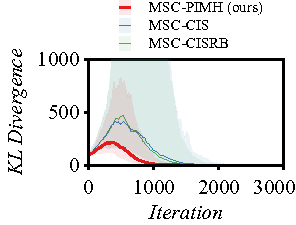
\includegraphics[scale=0.85]{figures/gaussian_01.pdf}
  }
  \subfloat[\(N=2^4\)]{
    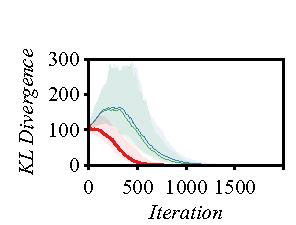
\includegraphics[scale=0.85]{figures/gaussian_02.pdf}
  }
  \subfloat[\(N=2^6\)]{
    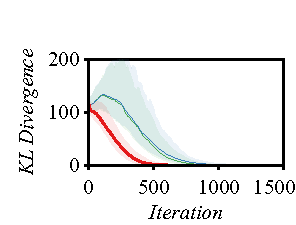
\includegraphics[scale=0.85]{figures/gaussian_03.pdf}
  }
  \caption{Inclusive KL minimization with a varying computational budget \(N\) on a 100-D isotropic Gaussian example.
    MSC with our proposed PIMH kernel (\textcolor{red}{red line}) converges faster than CIS with (\textcolor{green}{green line}) and without (\textcolor{blue}{blue line}) Rao-Blackwellization regardless of \(N\).
    Also, the convergence of MSC-PIMH becomes more stable/monotonic as \(N\) increases.
    The solid lines are the median of 100 repetitions while the colored regions are the 80\% empirical percentiles.
  }
\end{figure}

\section{Logistic Regression}


\begin{figure}
  \centering
  \subfloat[Pima]{
    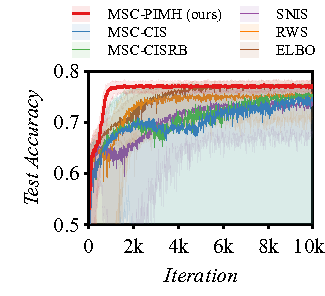
\includegraphics[scale=0.80]{figures/pima_02.pdf}
  }
  \subfloat[Heart]{
    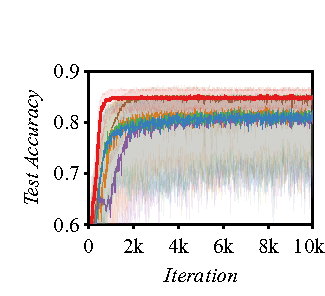
\includegraphics[scale=0.80]{figures/heart_02.pdf}
  }
  \subfloat[German]{
    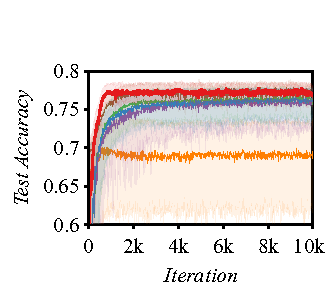
\includegraphics[scale=0.80]{figures/german_02.pdf}
  } \\
  \subfloat[Pima]{
    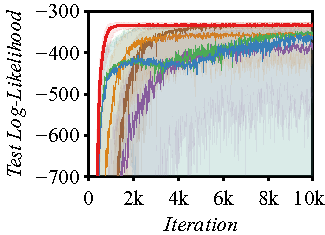
\includegraphics[scale=0.80]{figures/pima_03.pdf}
  }
  \subfloat[Heart]{
    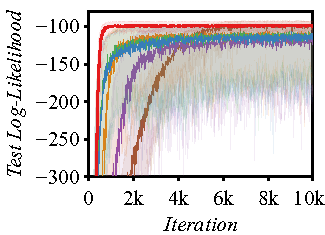
\includegraphics[scale=0.80]{figures/heart_03.pdf}
  }
  \subfloat[German]{
    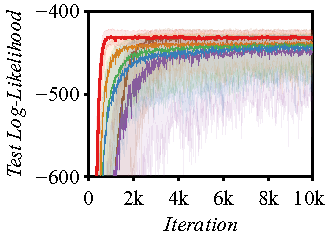
\includegraphics[scale=0.80]{figures/german_03.pdf}
  }
  \caption{Test accuracy and log-likelihood of logistic regression problems.
    The solid lines are the median of 100 repetitions while the colored regions are the 80\% empirical percentiles.
  }
\end{figure}

\paragraph{Did inclusive VI live up to its hype?}
\citet{dhaka_challenges_2021} showed that, inclusive VI works against our intuitions in higher dimensions.
However, if the posterior is strongly correlated, inclusive VI can fail even in lower dimensions.
On the other hand, if the posterior is not strongly correlated, our experiments suggest that inclusive VI can work better than exclusive VI.
Furthermore, posterior correlation affects all methods relying on the mean-field approximation, not only inclusive VI.

%A practical question would be to ask how correlated are problems encountered in practice
%%% Local Variables:
%%% TeX-master: "master"
%%% End:
